\section{Milestones}
\label{ProjMgmtMilestones}

Todo,
Work for Future Roland
He will have to describe the milestones

 

The following phase are defining blocks which can be closed after completing each and move on. The conclusion and start of each phase are used to review and adapt the current state.
The milestones are events during the course of the phases. Each milestone will be documented if it has been reached in time. Furthermore, any adaptions required to the milestone plans have to be documented.


The milestone timelines are setup as follows before project start.

\begin{itemize}
    \item Milestone 1, use case defined: 18.10.2026
    \item Milestone 2, Stakeholder meetings held: 15.11.2026
    \item Milestone 3, Error documentation by stakeholders started: 29.11.2026
    \item Milestone 4, Development environment set, initial setup of tools: 13.12.2026
    \item Milestone 5, MVP has been setup: 21.03.2027
    \item Milestone 6, MVP presented to Post stakeholders: 04.04.2027
    \item Milestone 7, Outline of second iteration defined: 18.04.2027
    \item Milestone 8, Data of different approaches compared: 16.05.2027
    \item Milestone 9, Thesis document completed: 11.07.2027
    \item Milestone 10, Presentation ready: 25.07.2027
\end{itemize}

\begin{figure}[H]
    \centering
    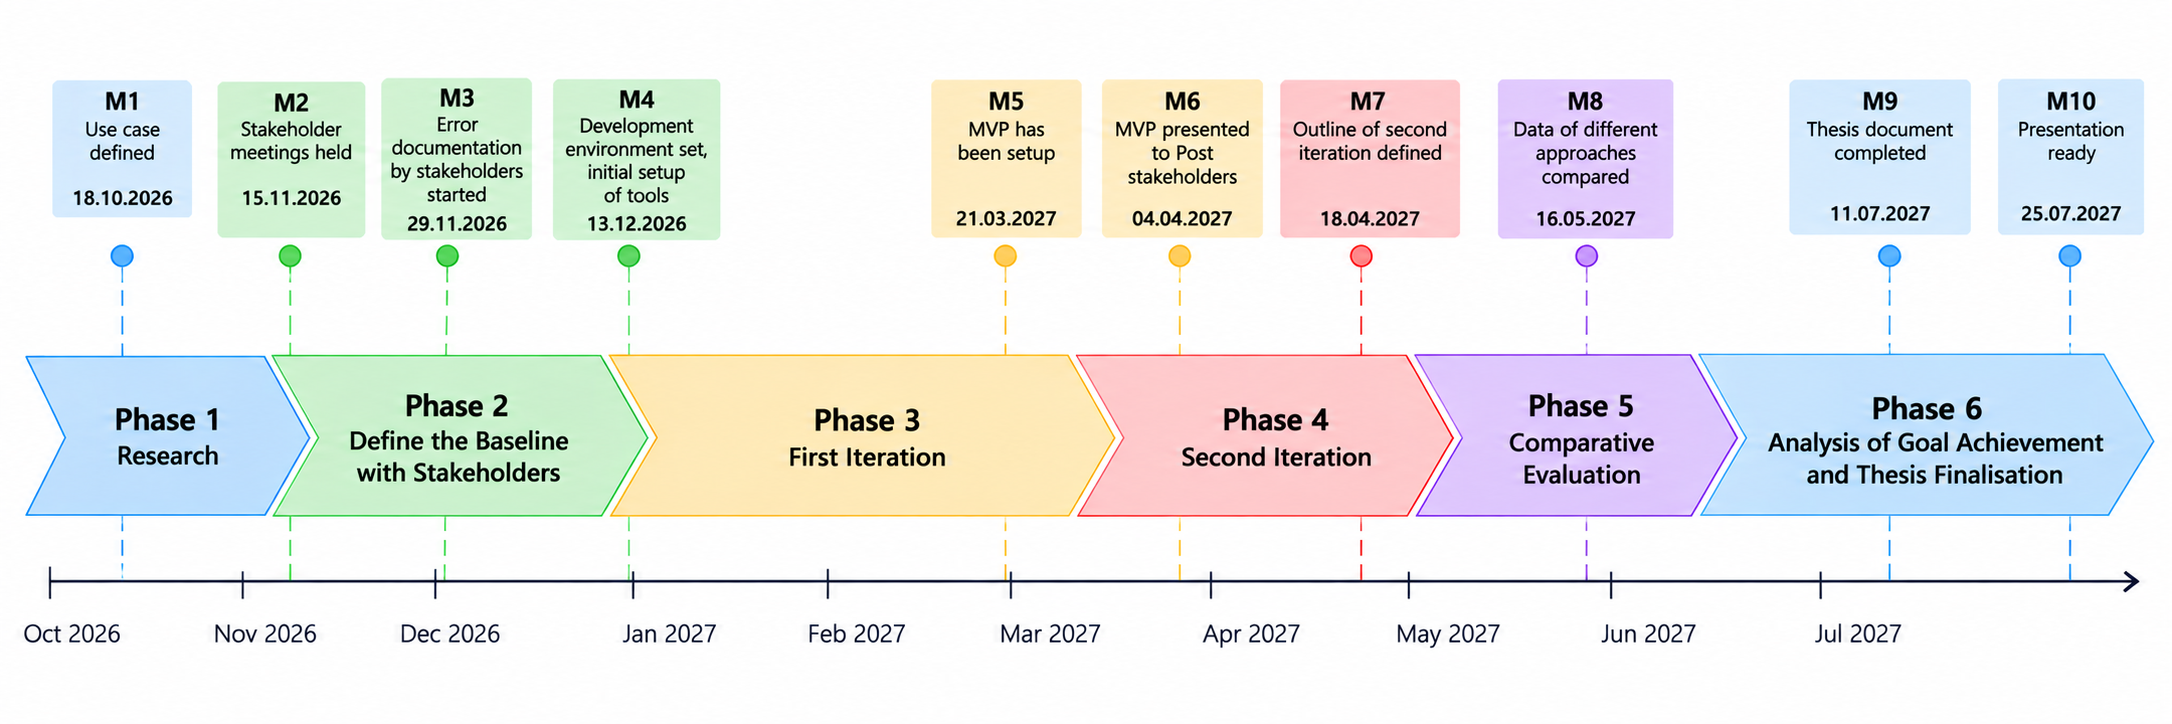
\includegraphics[width=0.8\textwidth]{./content/img/Mth/ProjectManagement/MilestoneTimelineAdapted_2.png}
    \caption{Milestones and phases defined at the start of the project}
    \label{fig:projmgmt_milestones_and_phases}
\end{figure}

